\chapter{Results}\label{chap5}
In this section we present the preliminary results of the performance of the $\tauh$ identification algorithm using $\int\mathcal{L} dt=139.2$ fb$^{-1}$ of data recorded between 2015 and 2018.
The correction factors are applied to simulation in order to match the efficiency observed in data. These correction factors are defined as the ratio between the efficiency measured in data and in simulation. For the present report, we present the value of the correction factors for \textit{Tight} ID working point for $\tauh$ candidates with $\pt$ above 45 GeV.

\section{$\mu\tau$ Final state}
We define the simulation correction factor as
\begin{equation}
	C_{\text{Tight-ID}}=\frac{\mathcal{E}_{\text{Data}}}{\mathcal{E}_{\text{MC}}}.
\end{equation}
The value obtained for the final state that contains one muon and a $\tauh$ candidate is

All the distributions of the relevant cuts for selecting our signal events after applying all the other cuts are shown in Fig.\ref{Fig17} (Appendix A).
\section{$e\tau$ Final state}
The value obtained for $C_{\text{Tight-ID}}$ in the final state that contains one electron and a $\tauh$ candidate is

All the distributions of the relevant cuts for selecting our signal events after applying all the other cuts are shown in Fig.\ref{Fig18} (Appendix A).
\section{Discussion}
As this study makes use of events highly boosted on the transverse plane the Z$(\pt)$ modelling is very important. In the first stages of our analysis we used Powheg+Pythia8 to simulate $Z\to\tauh l$ events. Fig.\ref{Fig23} shows the Z$(\pt)$ and $\Delta\phi(\tauh,l)$ for the muon-tau final state for in between events. As it can be seen the tendency in the MC is to underestimate the data for high-Z$(\pt)$ values. These results have been previously reported by ATLAS studies \cite{Aad:2019wmn}, and Fig.\ref{Fig20} shows the Z$(\pt)$ modelling made by different generators. This has motivated us to use Sherpa to simulate our signal events. The Z$(\pt)$ results for this generator are shown in Fig.\ref{Fig19} and there is improvement for high-$\pt$ values over Powheg+Pythia8. The complete set of plots showing the Z$(\pt)$ distribution for both e-tau and mu-tau final states for the two different type of topologies are shown in Fig.\ref{Fig21} and Fig.\ref{Fig22}.
\begin{figure}[ht]
	\centering
	\subfloat[]{\label{Fig23a}{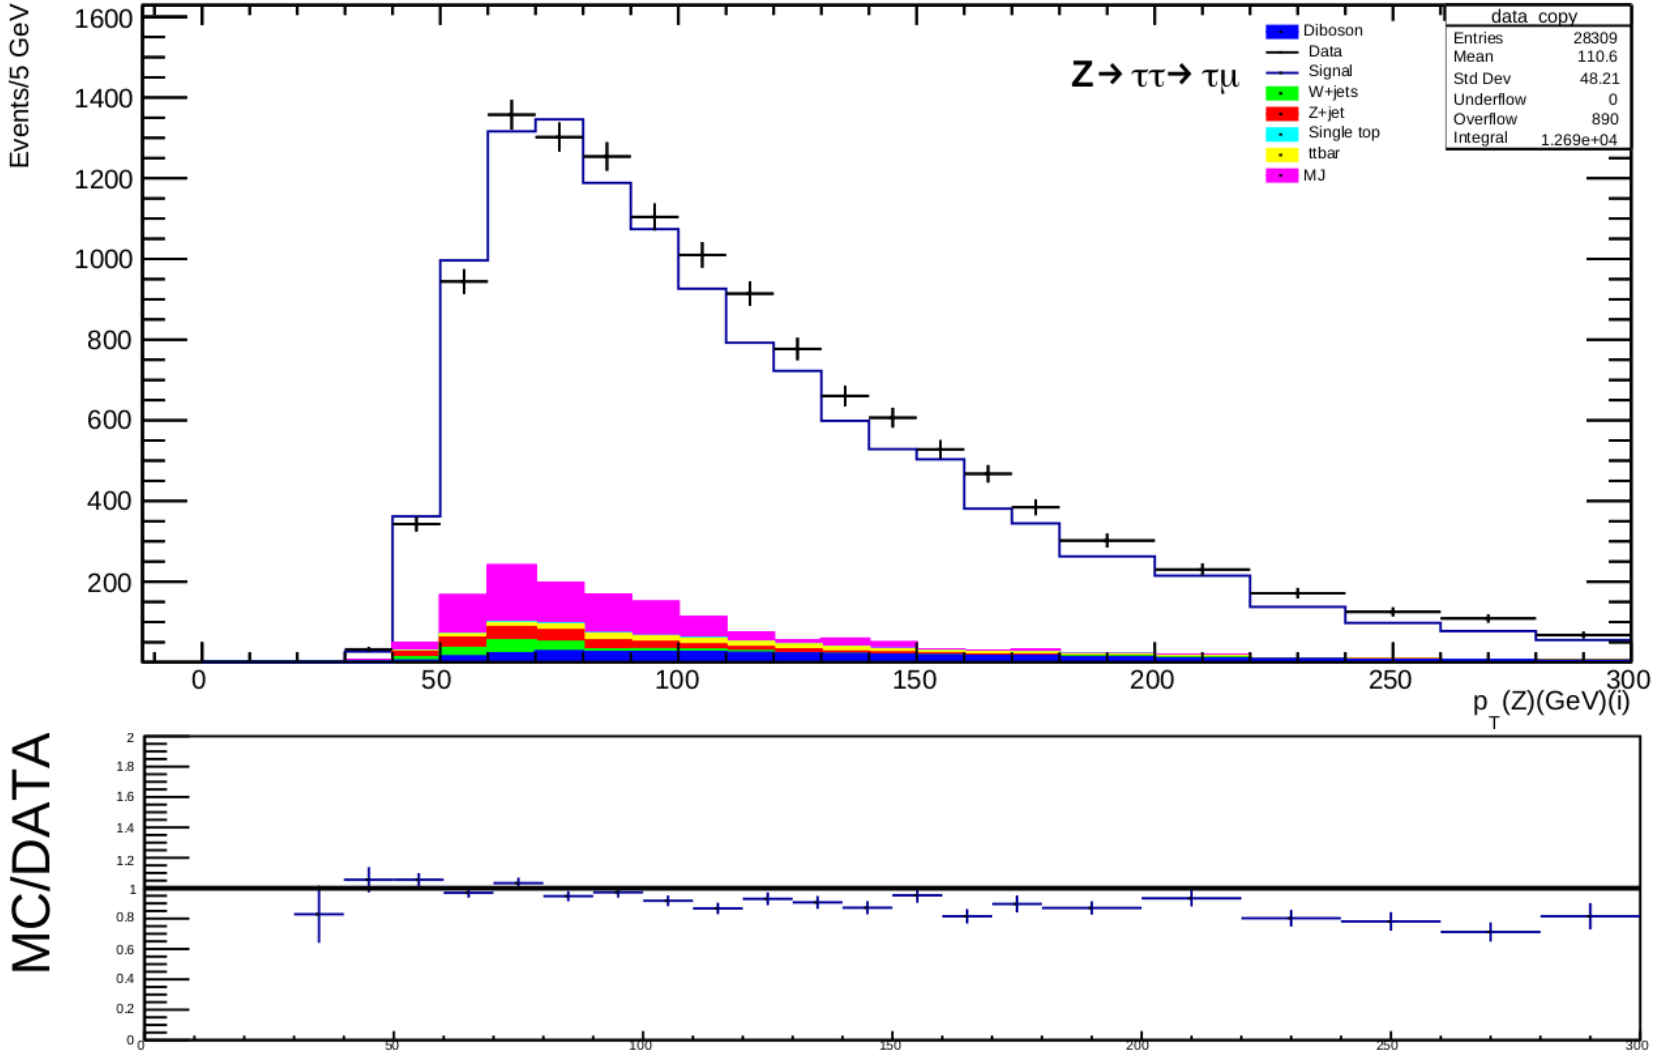
\includegraphics[width=0.50\textwidth]{figures/Fig23a}}}\hfill
	\subfloat[]{\label{Fig23b}{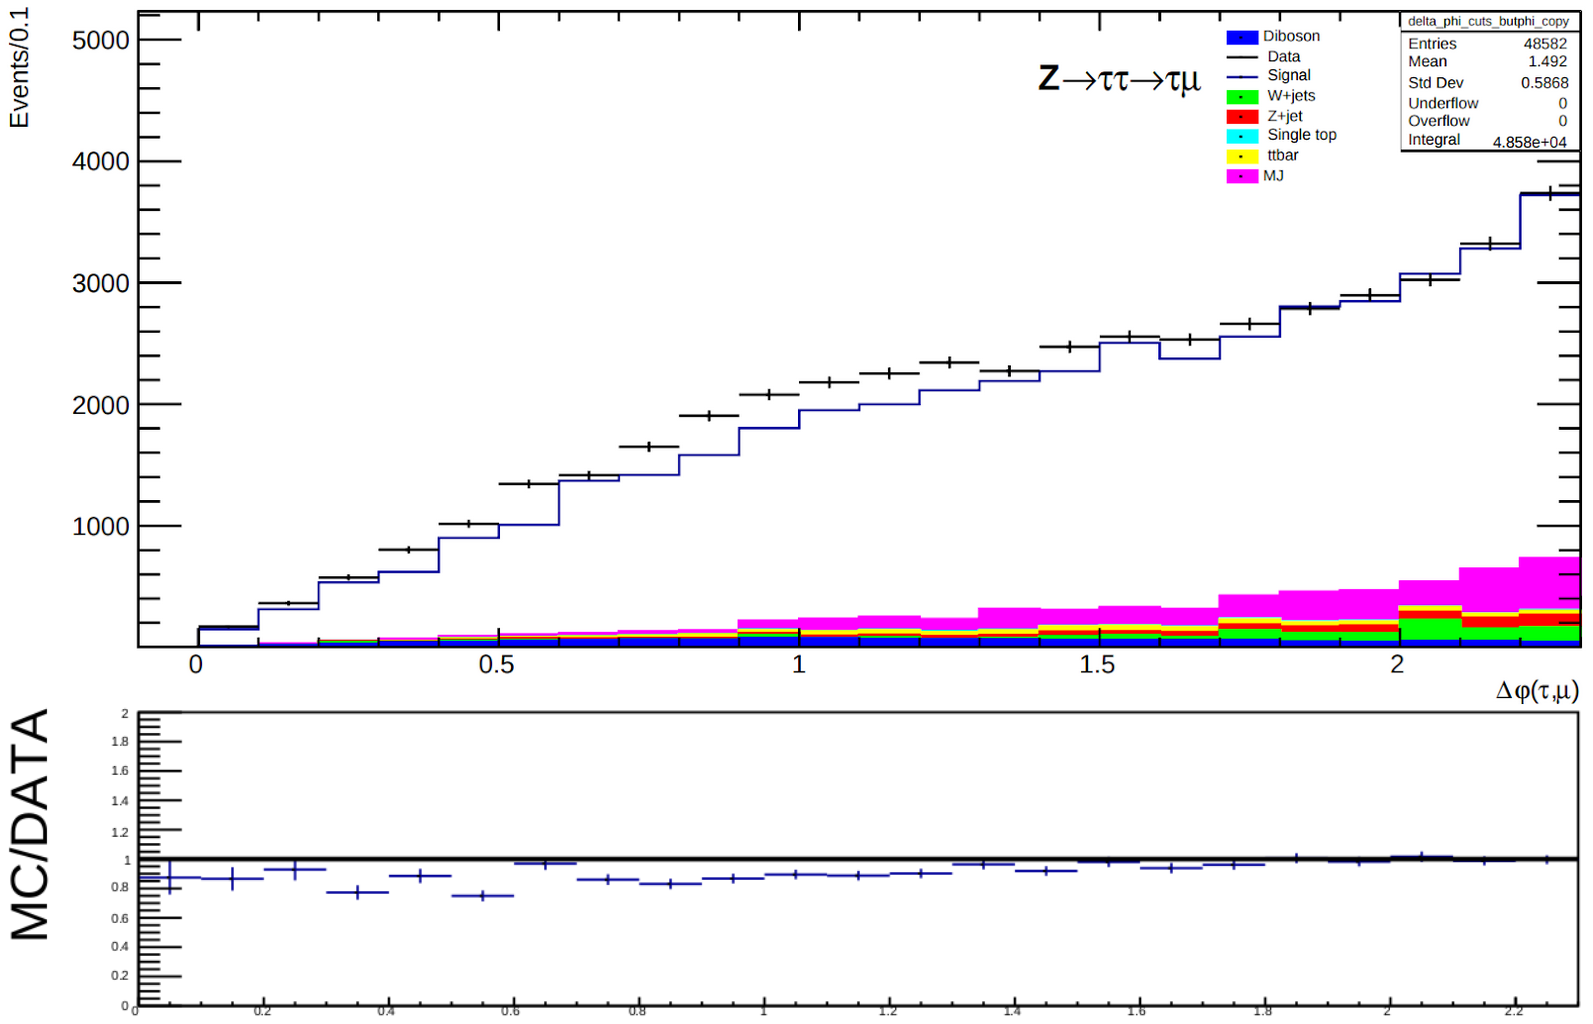
\includegraphics[width=0.50\textwidth]{figures/Fig23b}}}
	\caption{Distribution of Z$(\pt)$ for in between events (a) and $\Delta\phi(\tauh,l)$ (b) using Powheg+Pythia8. All the other cuts have been applied apart from the one being plotted.}
	\label{Fig23}
\end{figure}
\begin{figure}[ht]
	\centering
	\subfloat[]{\label{Fig19a}{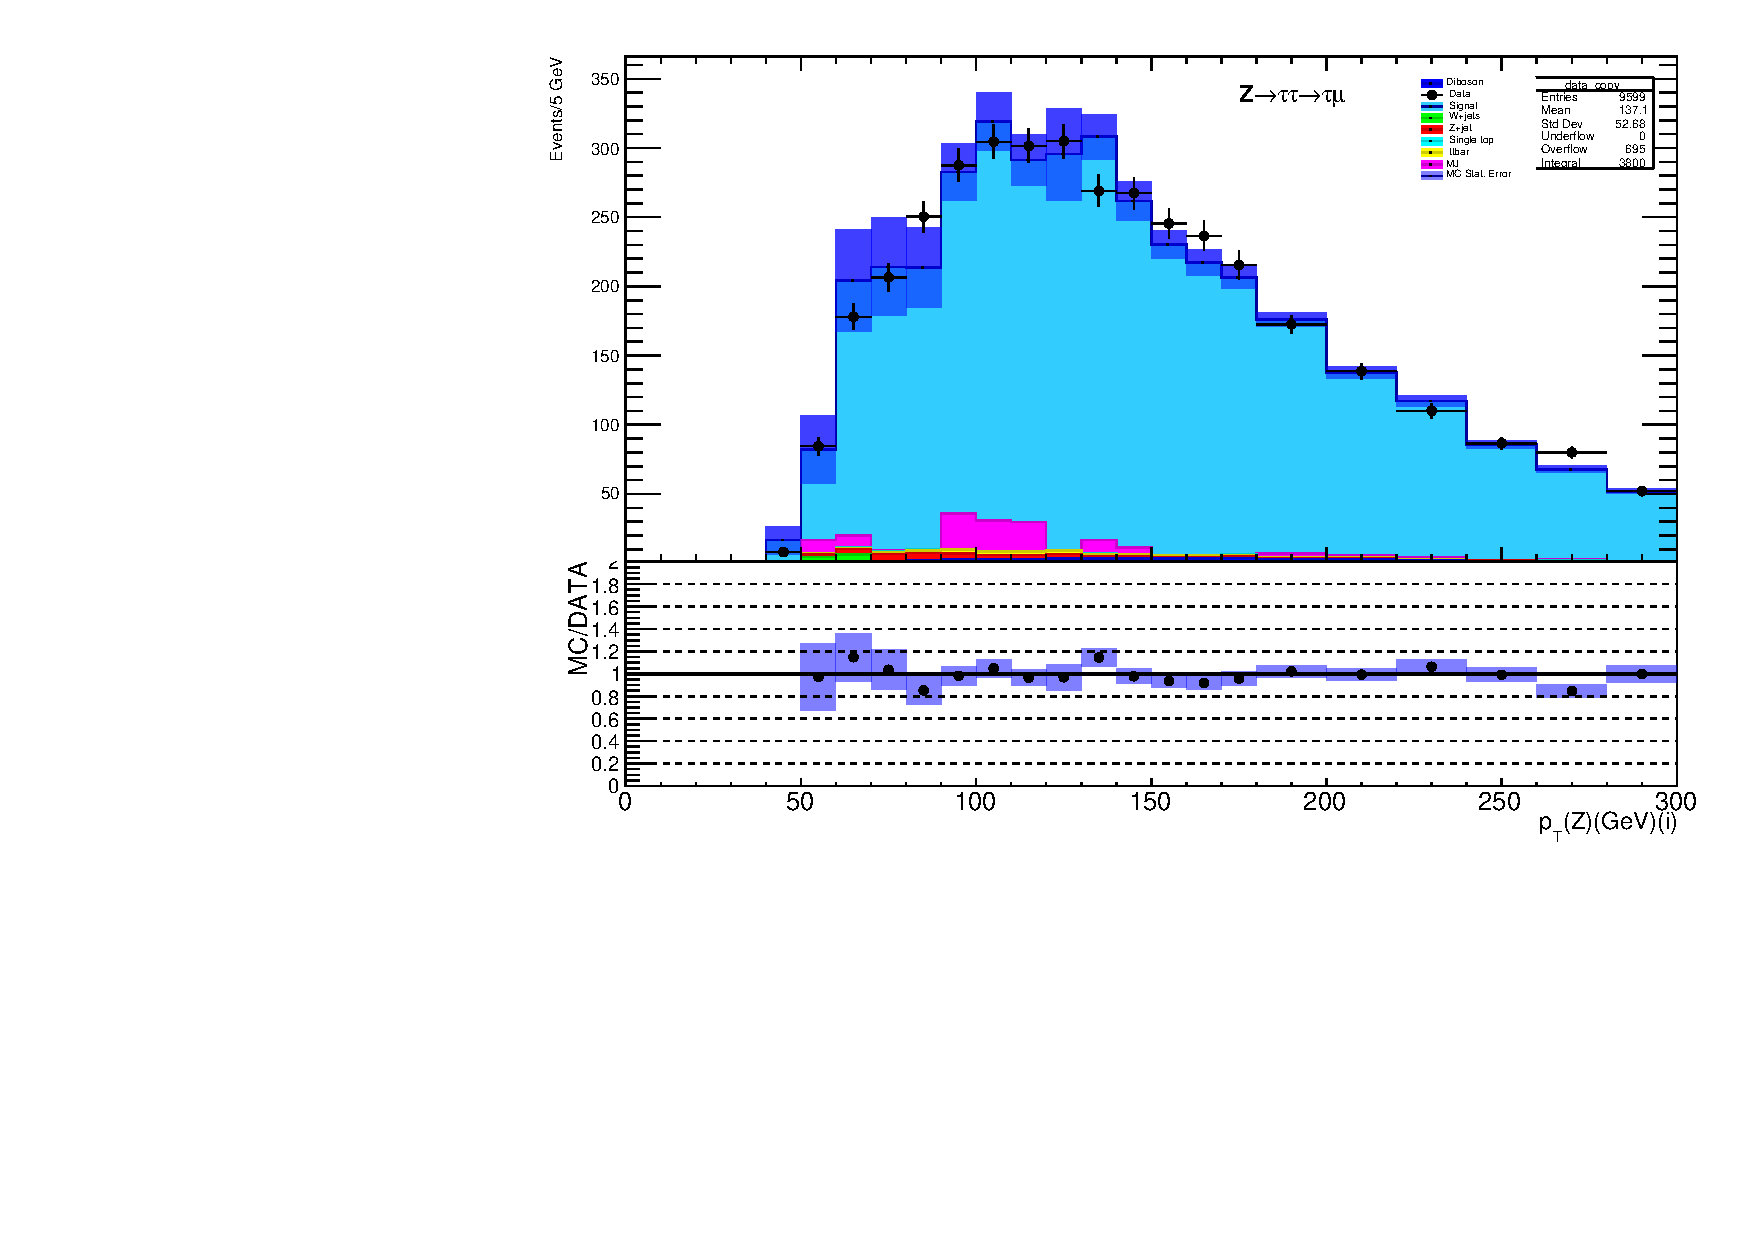
\includegraphics[width=0.50\textwidth]{figures/Fig19a}}}\hfill
	\subfloat[]{\label{Fig19b}{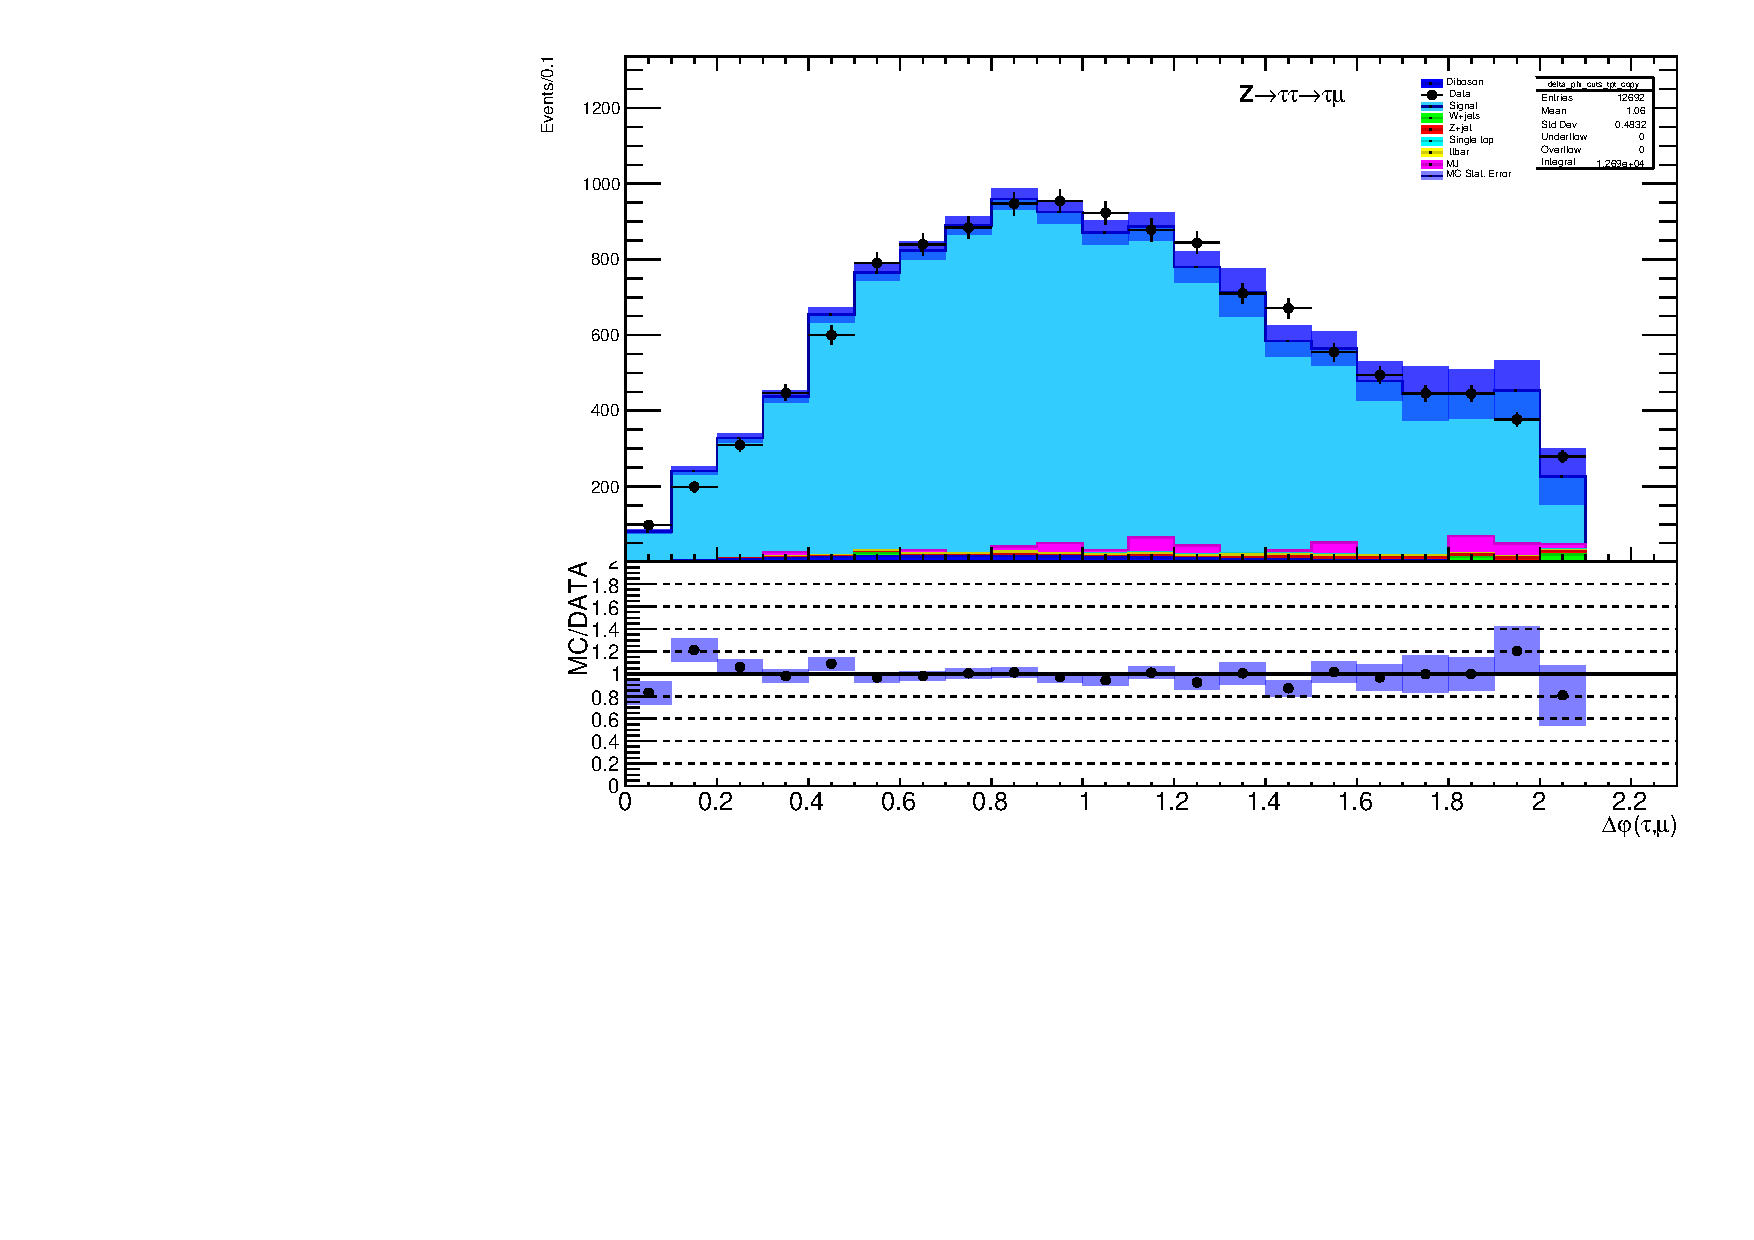
\includegraphics[width=0.50\textwidth]{figures/Fig19b}}}
	\caption{Distribution of Z$(\pt)$ for in between events (a) and $\Delta\phi(\tauh,l)$ (b) using Sherpa. All the other cuts have been applied apart from the one being plotted.}
	\label{Fig19}
\end{figure}
\begin{figure}[h]
	\centering
	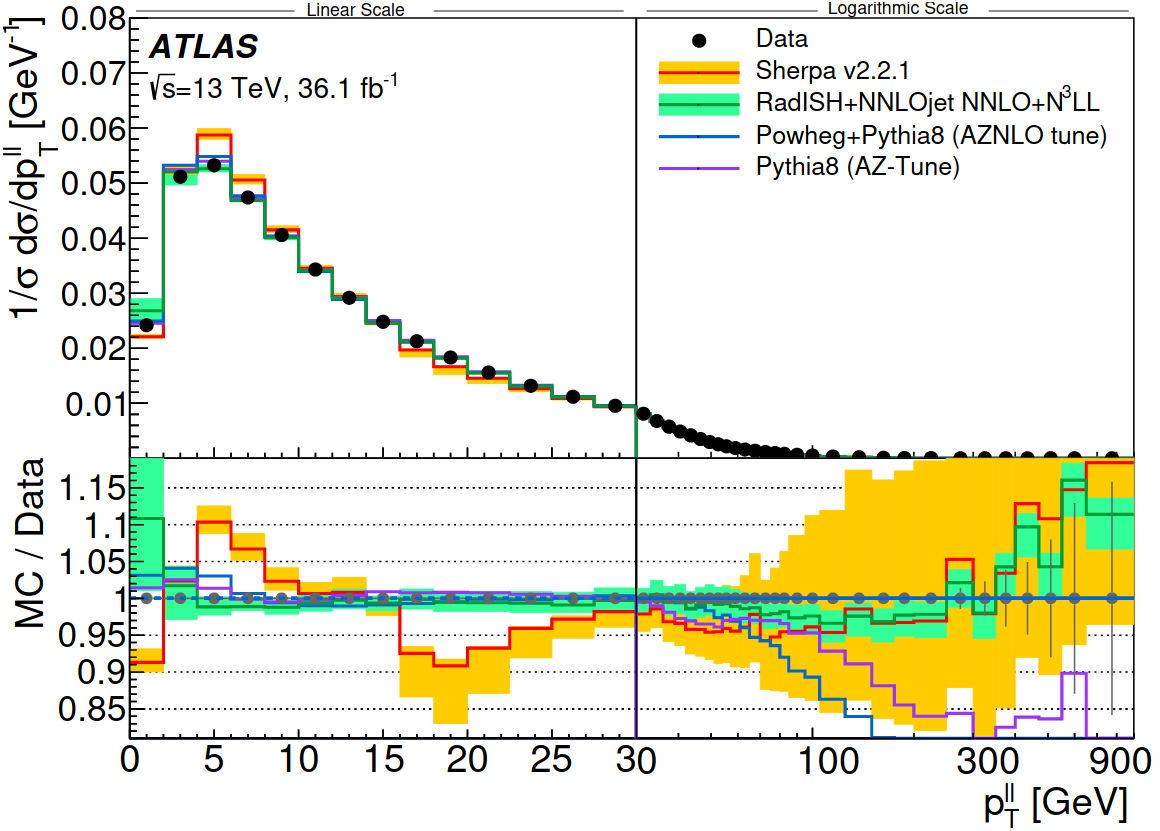
\includegraphics[width=0.5\textwidth]{figures/Fig20}
	\caption{Diagram showing the regions defined to estimate MJ background contribution in the SROS region. This data-driven method is also known as ABCD method.}
	\label{Fig20}
\end{figure}

Another challenging 